
The three mathematical evaluation scores mentioned in section \ref{section:TheoryEvaluatingClusteringResults}, i.e. Silhouette Coefficient, Davies-Bouldin Index, and Caliński-Harabasz Index, were used to compare the resulting clusters.  They were each implemented using the sklearn library, the same way as in section \ref{section:experimentTSNE}. These three scores were calculated and stored for each DataFrame, after each clustering algorithm was applied (DBSCAN and OPTICS) for each time length. The resulting values were then compared and are detailed in this section.

The experiment was run on each time length (\textit{1h files:} 15 min, 30 min, 45 min, 1h; \textit{3h files:} 30 min, 1h, 1 h 30 min, 2h, 2h 30 min, 3h).
The numbers were different for each time the results were calculated, since t-SNE produces slightly different results. Therefore, the t-SNE and clustering was run multiple times and the results were compared. In appendix \ref{appendix:clusteringEvaluationResults} figures \ref{figure:clusteringResults1} and \ref{figure:clusteringResults2}, two individual t-SNE and clusterings were run, figure \ref{figure:clusteringResults3} depicts the average scores of these two. Figure \ref{figure:clusteringResults4} depicts an average of a different two runs. These mentioned runs all held the learning rate parameter 20. Since a learning rate of 800 also proved to be a viable choice, the t-SNE and clustering was also run twice and averaged with this learning rate (figure \ref{figure:clusteringResults5}). The mean was taken from all these results, thus creating figure \ref{figure:clusteringResults6} (this figure can be seen in this section). From these, there is no clear winner, although there are some stronger candidates, i.e. 15 min (1h), 1h (1h), and 2h (3h). 

Like in section \ref{section:experimentTSNE}, when comparing the t-SNE results, the green fields indicate the best and most distinct clusters from the 1h or 3h data files, while the dark green fields also highlight the best value for that score overall for all time lengths (over all datasets). The green fields from all the above mentioned results, or number of wins, were summed to see which time length had the best number of scores the most times. The wins per dataset (1h or 3h - all green fields) for the 1h data files are pictured in figure \ref{figure:clusteringResultsGraph1h}, in figure \ref{figure:clusteringResultsGraph3h} for the 3 hour data files. The two top winners for the 1h data files and the 3h data files, were: 15 min (1h), 30 min (1h), 2h (3h), and 1h (3h). Figure \ref{figure:clusteringResultsGraphTotal} shows the comparison of the dark green wins (1h and 3h). The top four results were: 30 min (1h), 1h (3h), 2h (3h), and 30 min (3h). The number of wins is to some extent reliable on the resulting scores from other time lengths it happened to be compared with. It also does not fully factor in the full extent of how far this time length was better. For this reason, time lengths that were among the stronger candidates at least once (either in figures \ref{figure:clusteringResults6}, \ref{figure:clusteringResultsGraph1h} and \ref{figure:clusteringResultsGraph3h}, or \ref{figure:clusteringResultsGraphTotal}) were compared solely to each other. The results are detailed in figure \ref{figure:clusteringResults8}. The 2h time delta achieved the majority of best scores in this final comparison. 

\begin{figure}
  \centering
  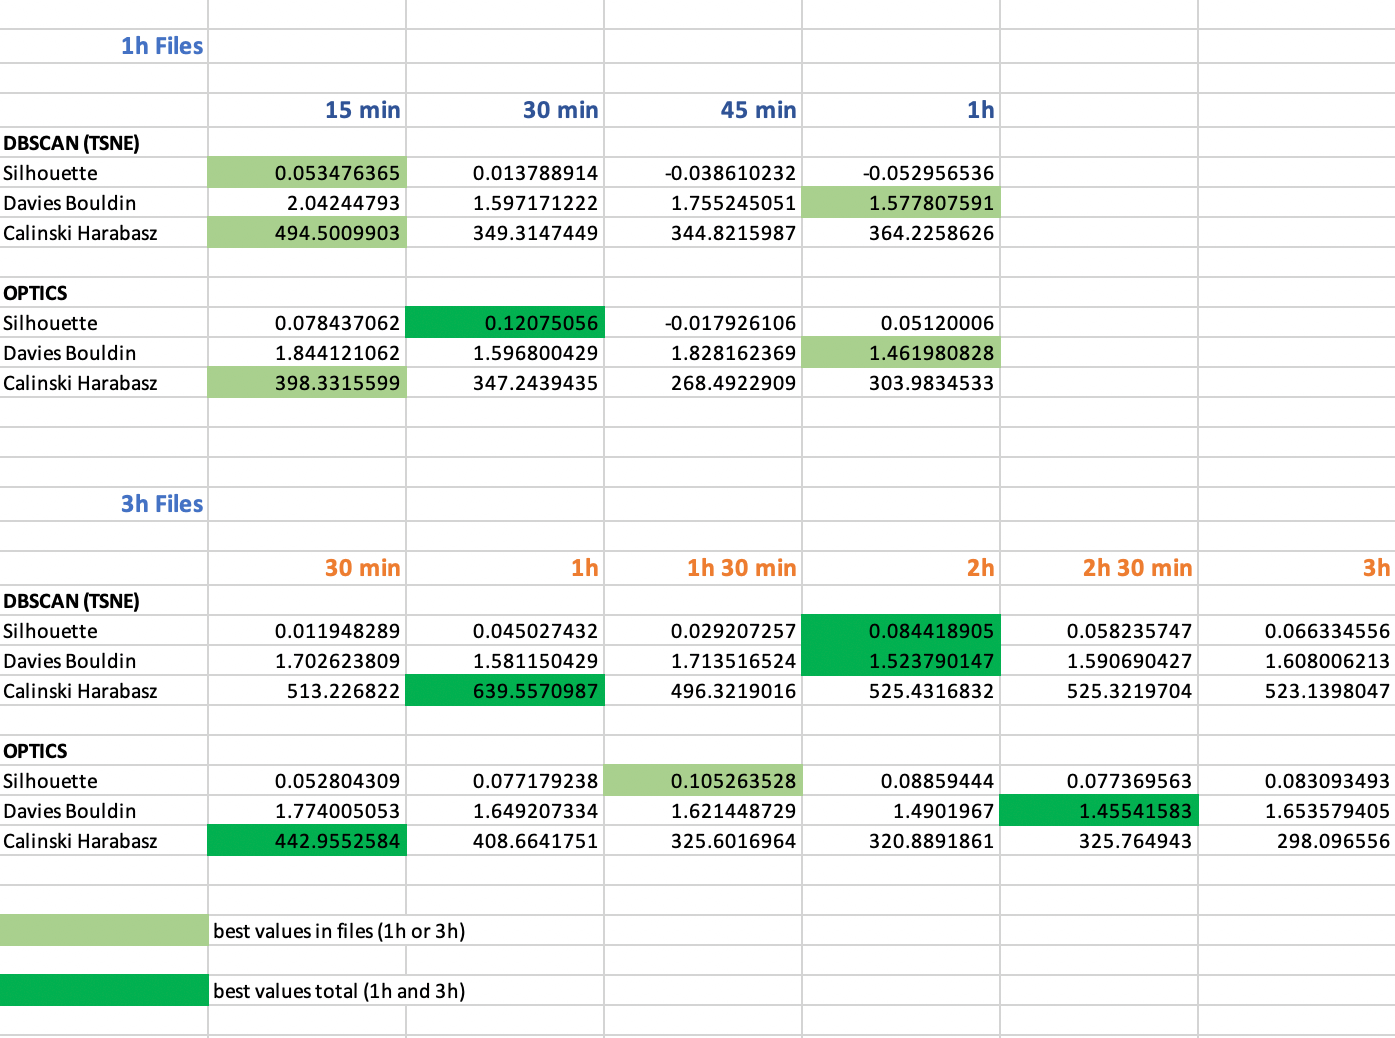
\includegraphics[width=0.8\textwidth]{./images/clusteringResults/clusteringResults6.png}
  \caption{Evaluation scores comparison averaged from figures \ref{figure:clusteringResults1}, \ref{figure:clusteringResults2}, \ref{figure:clusteringResults3}, \ref{figure:clusteringResults4}, and \ref{figure:clusteringResults5}. The lighter green highlighted values indicate the best values of that file aggregation (1h or 3h files). The dark green highlighted values illustrate the overall best values over all files (1h and 3h files). The time lengths with the highest number of wins includes 15 min (1h), 1h (1h), and 2h (3h). }
  \label{figure:clusteringResults6}
\end{figure}


\begin{figure}
  \centering
  \begin{subfigure}{.475\textwidth}
    \centering
    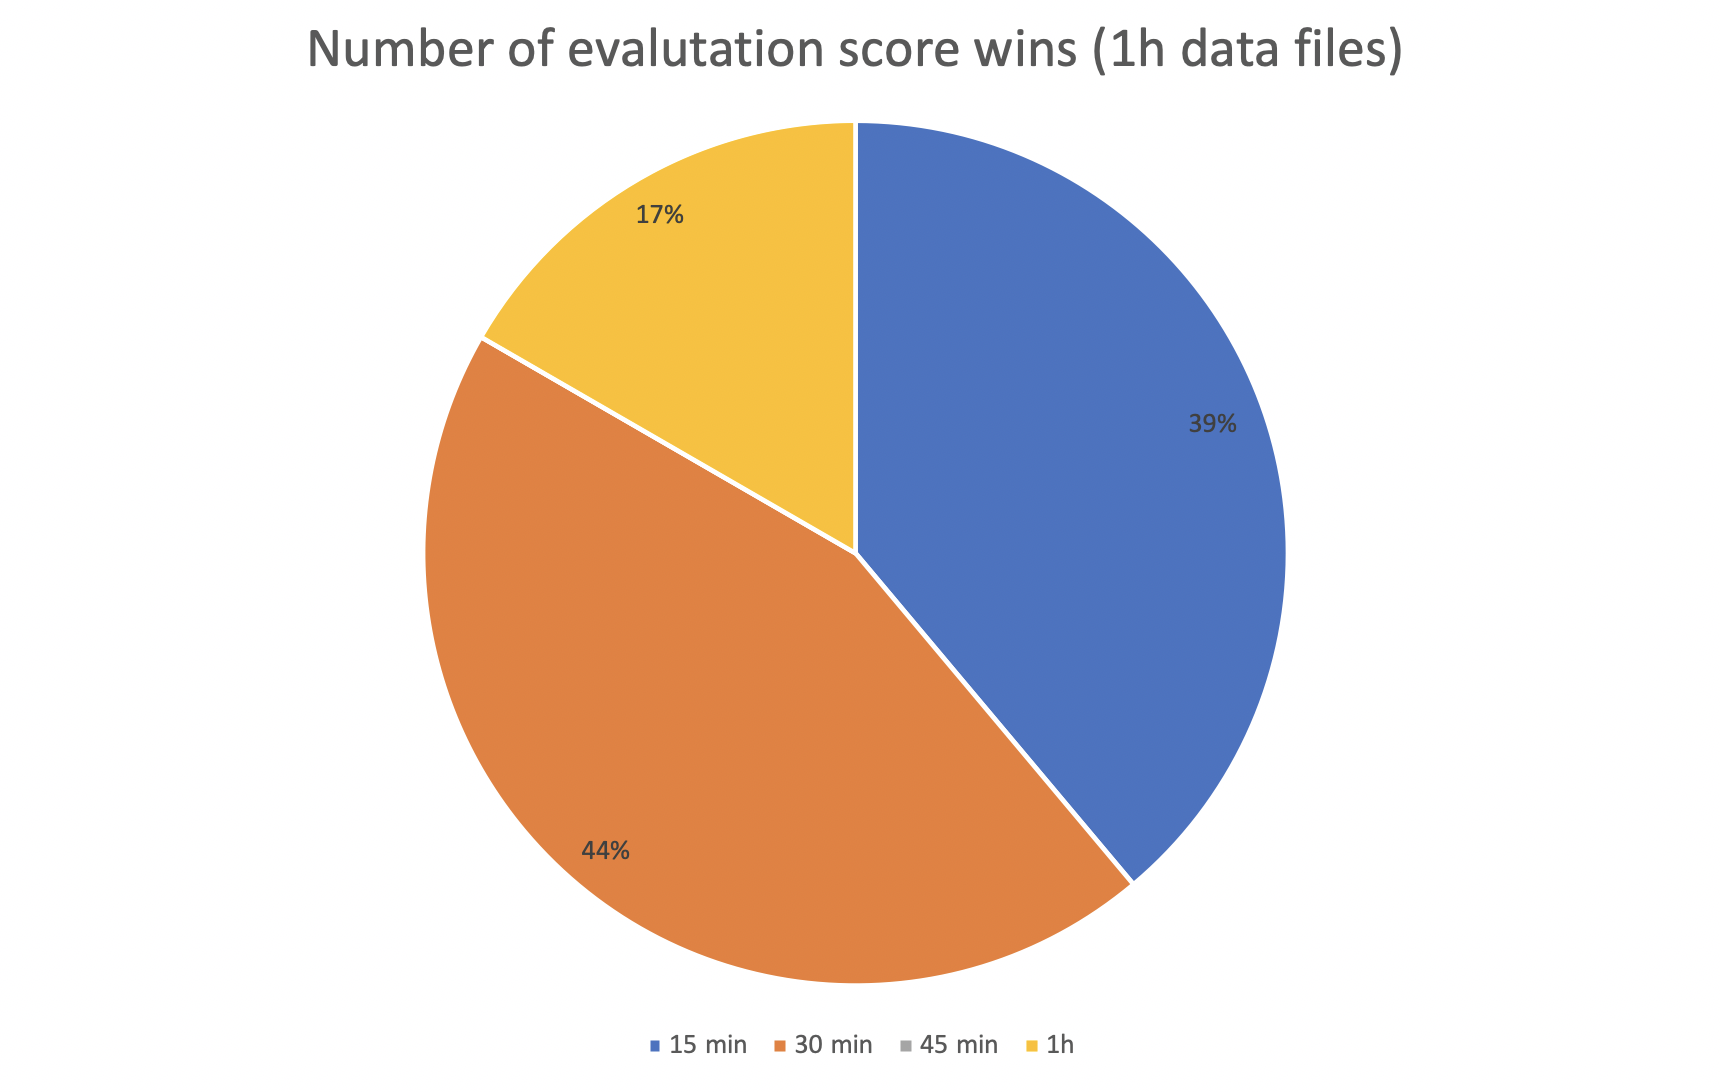
\includegraphics[width=1\textwidth]{./images/clusteringResults/clusteringResultsGraph1h.png}
    \caption{Number of evaluation score wins (1h or 3h dataset) for the 1h data files.}
    \label{figure:clusteringResultsGraph1h}
  \end{subfigure}
  \hfill
  \begin{subfigure}{.475\textwidth}
    \centering
    \  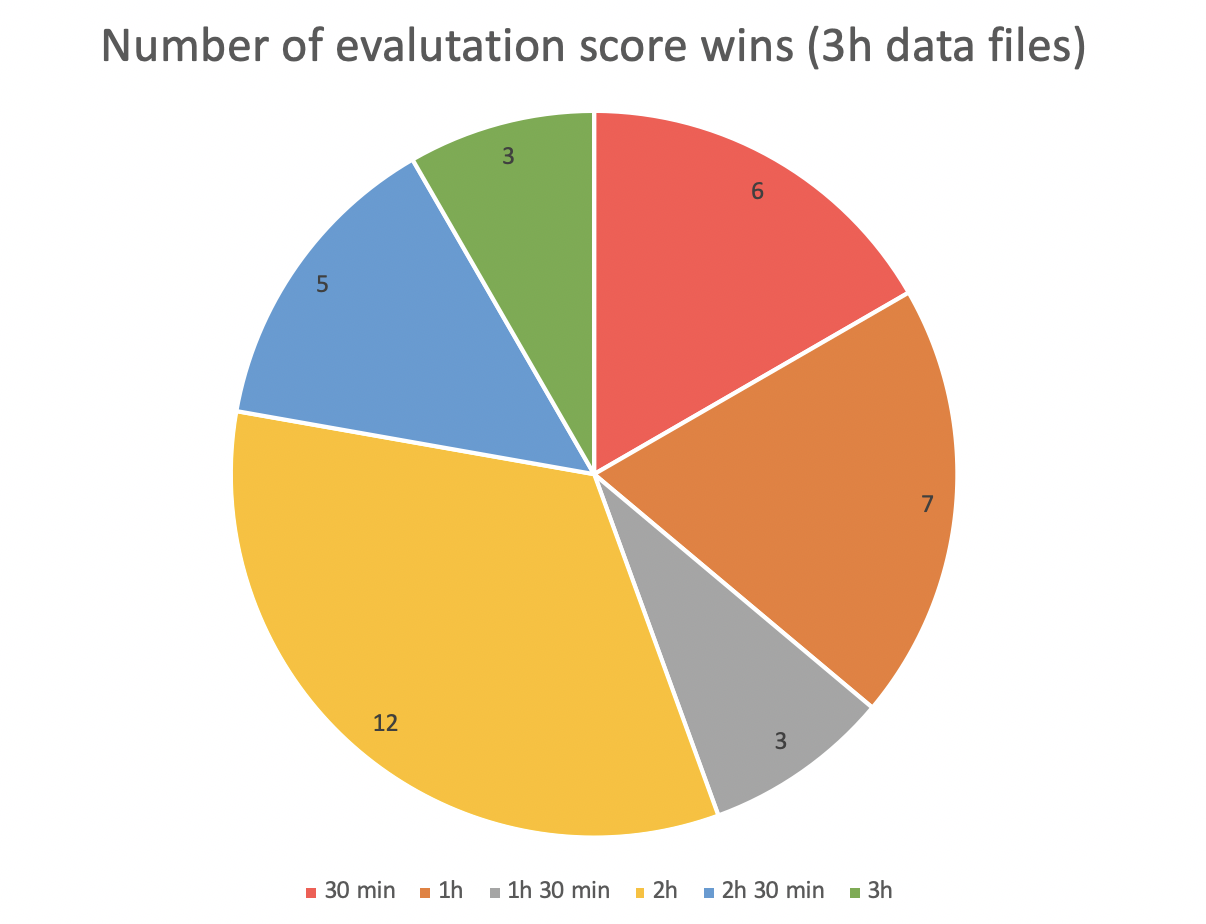
\includegraphics[width=1.2\textwidth]{./images/clusteringResults/clusteringResultsGraph3h.png}
    \caption{Number of evaluation score wins (1h or 3h dataset) for the 3h data files.}
    \label{figure:clusteringResultsGraph3h}
  \end{subfigure}
\end{figure}

\begin{figure}
  \centering
  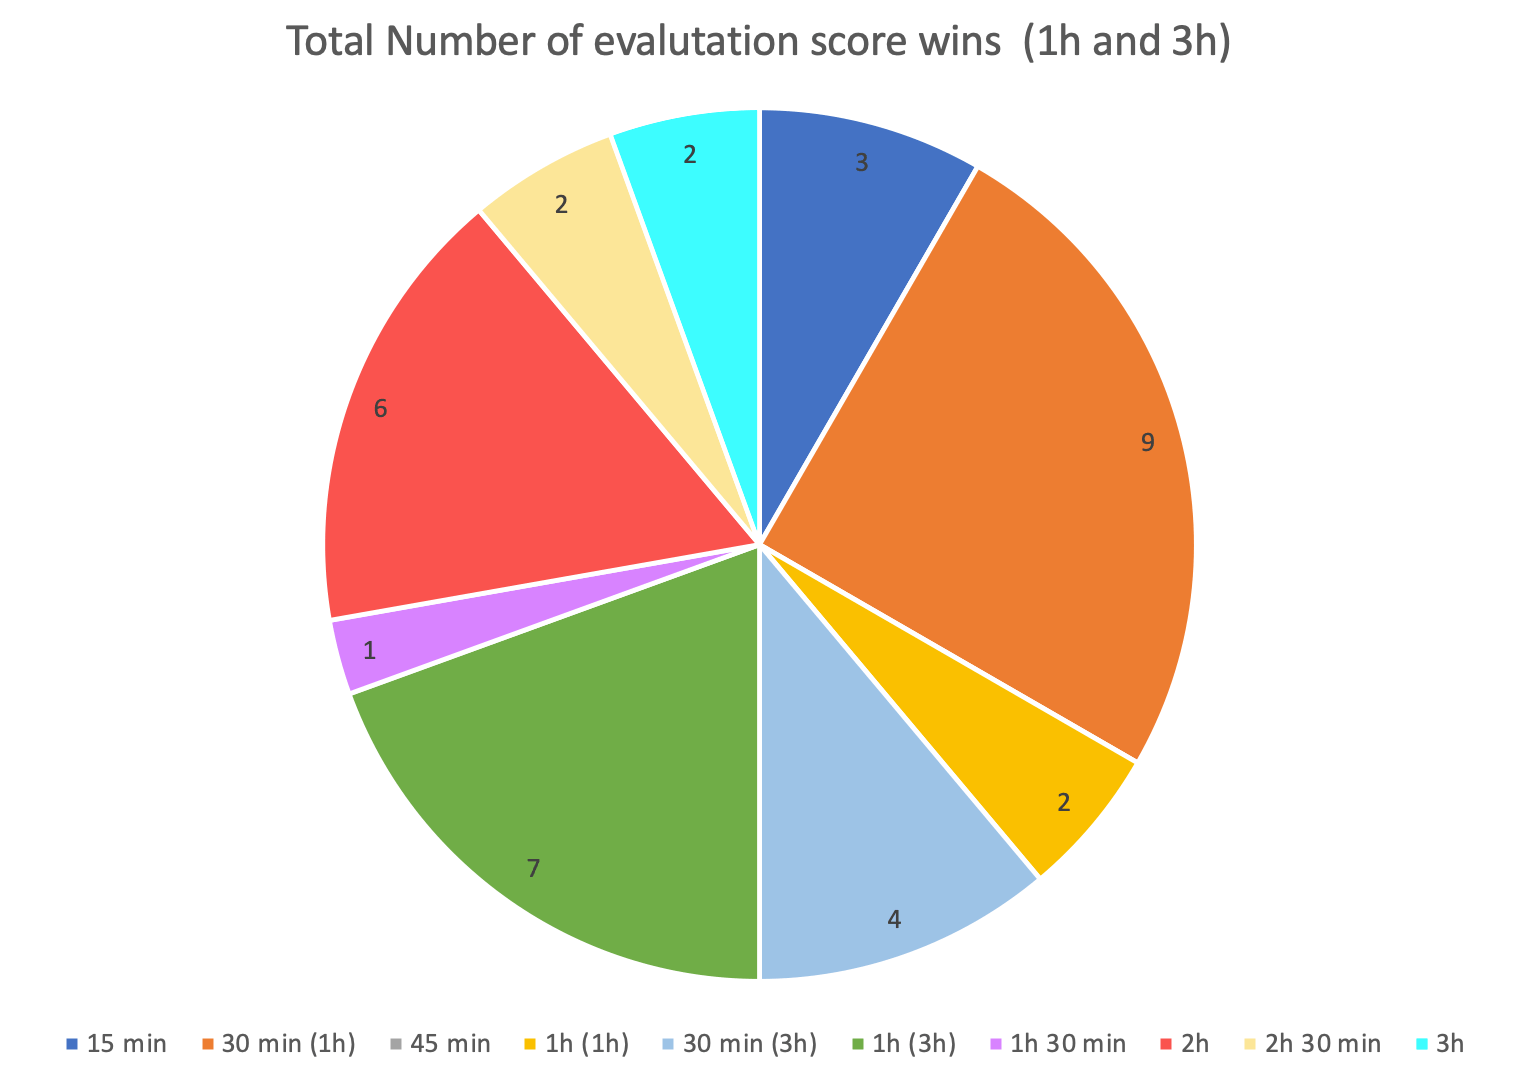
\includegraphics[width=0.7\textwidth]{./images/clusteringResults/clusteringResultsGraphTotal.png}
  \caption{Number of dark green evaluation score wins (1h and 3h dataset).}
  \label{figure:clusteringResultsGraphTotal}
\end{figure}

\begin{figure}
  \centering
  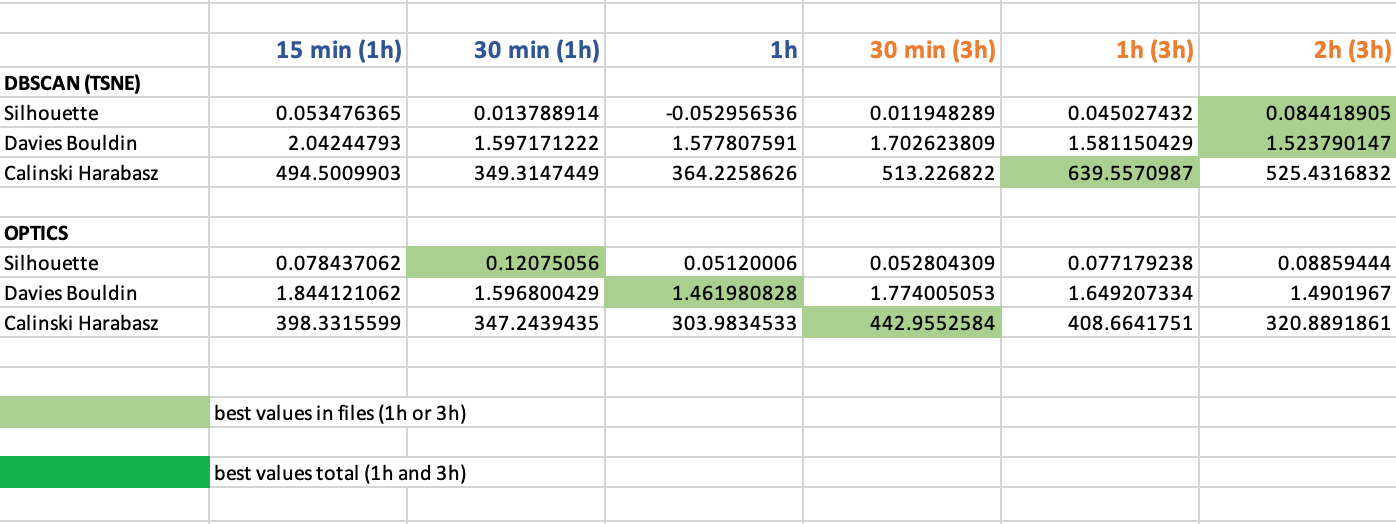
\includegraphics[width=0.8\textwidth]{./images/clusteringResults/clusteringResults8.png}
  \caption{Comparison of top evaluation score performers (of clusterings) from figures \ref{figure:clusteringResultsGraph1h}, \ref{figure:clusteringResultsGraph3h}, and \ref{figure:clusteringResultsGraphTotal}. The light green highlighted cells indicate the best value across the different time lengths for that score.}
  \label{figure:clusteringResults8}
\end{figure}

\clearpage
